\documentclass[12pt]{article}

\usepackage{amsmath,amsthm,amsfonts,amssymb,amsxtra}
\usepackage{tikz,array}
\usetikzlibrary{arrows}
\renewcommand{\theenumi}{(\alph{enumi})} 
\renewcommand{\labelenumi}{\theenumi}

\pagestyle{empty}
\setlength{\textwidth}{7in}
\setlength{\oddsidemargin}{-0.5in}
\setlength{\topmargin}{-1.0in}
\setlength{\textheight}{9.5in}

\theoremstyle{definition}
\newtheorem{problem}{Problem}

\begin{document}

\noindent{\large\bf MATH 242}\hfill{\large\bf Final Exam}\hfill{\large\bf
Spring 2018}\hfill{\large\bf Page 1/3}\hrule

\bigskip
\begin{center}
\begin{tabular}{|ll|}
\hline & \cr
{\bf Name: } & \makebox[12cm]{\hrulefill}\cr & \cr
{\bf VIP ID:} & \makebox[12cm]{\hrulefill}\cr & \cr
\hline
\end{tabular}
\end{center}
\begin{itemize}
  \item Write your name and your VIP ID in the space provided above.
  \item You have 150 minutes (2.5 hours) to complete the exam.
  \item Show sufficient work to justify all answers unless otherwise stated in the problem.  Correct answers with inconsistent work may not be given credit.
  \item You must show proficiency solving theoretical questions on differential equations---each of the parts in Problem \#1.  Each of these differential equations are graded as follows:
  \begin{center}
  \begin{tabular}{|l|c|}
  \hline
  Perfect solution & 5 pts \\ \hline
  Arithmetic errors, everything else correct & 4 pts \\ \hline
  Correct treatment of the differential equation, poor integration & 2 pts \\ \hline
  Incorrect treatment of the differential equation, or bad algebra & 0 pts \\ \hline
  \end{tabular}
  \end{center}
  If the combined score of Problem \#1 is not at least 35 points, none of the application problems will be graded.
\end{itemize}
\hrule

\begin{center}
\begin{tabular}{|l|r|c|} \hline
             & Points & Score \\ \hline \hline
             &        &  \\
\Large Theory       &  \Large 50    &  \\ && \\ \hline
             &        &  \\
\Large Applications &  \Large 50    &  \\ && \\ \hline \hline
             &        &  \\
\Large Total        & \Large100    &  \\ && \\ \hline
\end{tabular}
\end{center}

\hrule

\vspace{0.6cm}

\begin{quotation}
\noindent I, \makebox[8cm]{\hrulefill}, have chosen to take the final exam for Section 005 of Math 242 in the Spring'18 session.  The grade I earn on this final exam will be my grade for the course and once I begin this exam, I must complete it.  I am hereby declining my option to take the grade I currently have in the course, and I realize that my final course grade, as determined by this final exam alone, may be lower than my current grade.  I realize this decision is final.

\vspace{1cm}

\noindent Student Signature: \makebox[8cm]{\hrulefill} Date: \makebox[3cm]{\hrulefill}


\end{quotation}
\newpage

%%%%%%%%%%%%%%%%%%%%%%%%%%%%%%%%%%%%% Page 2
\noindent{\large\bf MATH 242}\hfill{\large\bf Final Exam}\hfill{\large\bf Spring 2018}\hfill{\large\bf Page 2/3}\hrule

\bigskip
\begin{problem}[50 pts--5 pts each part]
Find a general solution to the following differential equations.
\begin{enumerate}
\item $(x^2-y^2)y'=2xy$
\item $(2x\sin y \cos y )y'+4x^2+\sin^2 y = 0$
\item $(x^2+4)y'+3xy-x=0$
\item $y''=(x+y')^2$
\item $yy''=3(y')^2$
\item $x^2y'+2xy=5y^4$
\item $y'=\sqrt{x+y+1}$
\item $y''+2y'+26y=82\cos 4x$
\item $y''+y=\tan x$
\item $y'=6e^{2x-y}$
\end{enumerate}
\end{problem}

\begin{problem}[10 pts]
A spherical bowl with radius 4~ft is full of water at time $t=0$.  At that moment a circular hole with diameter 1~in.~is opened in the bottom of the tank.  How long will it take for all the water to drain from the tank?
\end{problem}

\begin{problem}[10 pts--5 pts each part]
A body with mass 0.5~kg is attached to the end of a spring that is stretched 2~m by a force of 10~N.  The mass and spring are attached to a dashpot that provides 1~N of resistance for each meter per second of velocity.  This is set in motion one meter to the right, and moving to the left at that time with an initial velocity of 5~m/s.
\begin{enumerate}
  \item Find the position function of the body.
  \item Indicate the amplitude, frequency, period of oscillation and time lag of this motion.
\end{enumerate}
\end{problem}

\begin{problem}[10 pts]
Find all curves for which the normal at point $(x,y)$ and the line joining the origin with that point form an isosceles triangle having its base on the $x$--axis.
\end{problem}

\begin{problem}[10 pts--5 pts each part]
Suppose that at time $t=0$, two thirds of a logistic population of 153,000 persons have heard a certain rumor, and that the number of those who have heard it is then increasing­ at the rate of 1000 persons per day. How long will it take for this rumor to spread to 75\% of the population?
\end{problem}

\begin{problem}[10 pts]
Consider a logistic population $P(t)$ of fish on a lake, measured in hundreds after $t$ years, with $k=3$ and $M=6$.  Suppose that 450 fish are \emph{harvested} annually (at a constant rate throughout the year).  If the lake is initially stocked with 375 fish, when will its population reach 90\% of the carrying capacity?
\end{problem}

\newpage

%%%%%%%%%%%%%%%%%%%%%%%%%%%%%%%%%% Page 8
\noindent{\large\bf MATH 242}\hfill{\large\bf Final Exam}\hfill{\large\bf Spring 2018}\hfill{\large\bf Page 3/3}\hrule

\bigskip
{\Large Formula Sheet}

\begin{center}
%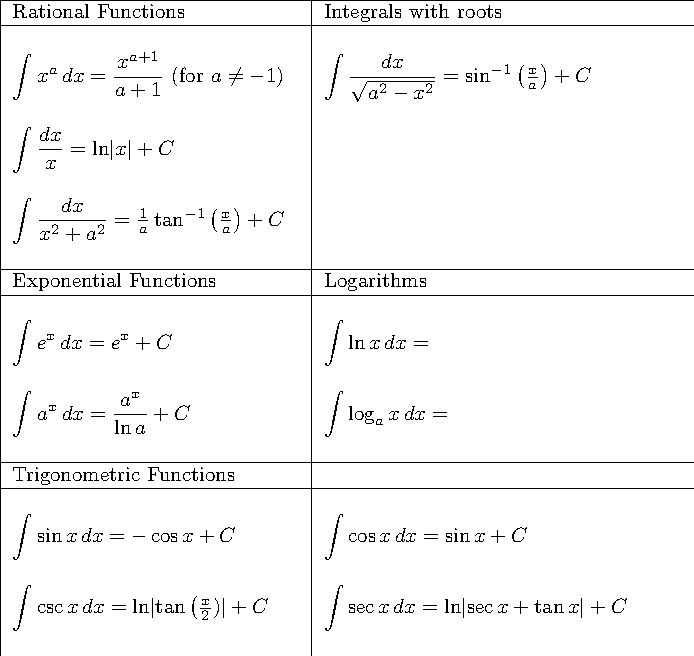
\includegraphics[width=\linewidth]{table.pdf}
\begin{tikzpicture}
  \node[scale=0.97]{
 \begin{tabular}{|m{1.2cm}|m{4.3cm}l||m{2.1cm}|m{4.3cm}l|}
 \hline
    $f(x)$\raisebox{0.5cm} & $\mathcal{L}\{f\}=\int_0^\infty e^{-sx}f(x)\, dx$\raisebox{0.5cm} & &
    \raisebox{0.5cm} & \raisebox{0.5cm} & \\[0.4cm] 
    \hline \hline
    $1$ & $\dfrac{1}{s}$\raisebox{0.6cm} & $s>0$ &
    $cf(x)\pm g(x)$ & $cF(s) \pm G(s)$\raisebox{0.4cm} & $s>max(a,b)$ \\[0.4cm]
    \hline
    $x^n$ & $\dfrac{n!}{s^{n+1}}$\raisebox{0.6cm} & $s>0$ & $e^{\alpha x}f(x)$ & $F(s-\alpha)$\raisebox{0.4cm} & $s>a+\alpha$ \\[0.4cm]
    \hline
    $e^{\alpha x}$ & $\dfrac{1}{s-\alpha}$\raisebox{0.6cm} & $s>\alpha$ &
    $x^n f(x)$ & $(-1)^n F^{(n)}(s)$\raisebox{0.4cm} & $s>a$ \\[0.4cm]
    \hline
    $\sin \beta x$ & $\dfrac{\beta}{s^2+\beta^2}$\raisebox{0.6cm} & $s>0$ & $f'(x)$ & $s F(s) -f(0)$\raisebox{0.4cm} & \\[0.4cm]
    \hline
    $\cos \beta x$ & $\dfrac{s}{s^2+\beta^2}$\raisebox{0.6cm} & $s>0$ &$f''(x)$\raisebox{0.4cm} & $s^2F(s) - sf(0)  - f'(0)$ & \\[0.4cm]
    \hline
    \end{tabular} };
    \end{tikzpicture}
\end{center}

\begin{itemize}
\item The slope of the tangent line to the curve at $(x_0,y_0)$ is $f'(x_0)$.
\item The slope of the normal line to the cure at $(x_0,y_0)$ is $-1/f'(x_0)$.
\item The equation of the tangent line at $(x_0,y_0)$ is $y-y_0=y'(x-x_0)$.
\item The equation of the normal line at $(x_0,y_0)$ is $y-y_0 = (x_0-x)/f'(x_0)$.
\item The $x$--intercept of the tangent is $x_0-f(x_0)/f'(x_0)$.
\item The $y$--intercept of the tangent is $f(x_0)-x_0 f'(x_0)$.
\item The $x$--intercept of the normal is $x_0+f(x_0)f'(x_0)$.
\item The $y$--intercept of the normal is $f(x_0)+x_0/f'(x_0)$.
\item The length of the tangent between $(x_0,y_0)$ and the $x$--axis is $\lvert y_0 \rvert\sqrt{1+1/f'(x_0)^2}$.
\item The length of the tangent between $(x_0,y_0)$ and the $y$--axis is $\lvert x_0 \rvert\sqrt{1+f'(x_0)^2}$.
\item The length of the normal between $(x_0,y_0)$ and the $x$--axis is $\lvert y_0 \rvert\sqrt{1+f'(x_0)^2}$.
\item The length of the normal between $(x_0,y_0)$ and the $y$--axis is $\lvert x_0 \rvert \sqrt{1+1/f'(x_0)^2}$.
\item The length of the subtangent is $\lvert f(x_0)/f'(x_0) \rvert$.
\item The length of the subnormal is $\lvert f(x_0) f'(x_0) \rvert$.
\end{itemize}

\end{document}